\documentclass[a4paper]{article}
\usepackage[swedish]{babel}
\usepackage[utf8]{inputenc}
\usepackage[T1]{fontenc}
\usepackage{graphicx}
\usepackage{float}
\setlength{\parindent}{0mm}
\setlength{\itemsep}{0ex}
\setlength{\parskip}{2ex}
\setlength{\parsep}{2ex}
\setlength{\partopsep}{0ex}
\setlength{\topsep}{0ex}

%---------------------------------------------------------------
\title{\bf \LARGE Lab report\\
Digital Design (EDA322)}

%\normalsize{
  %\begin{tabular}{|l|l|l|}  \hline
              %& \bf Namn                           & \bf Datum   \\ \hline \hline
     %Granskad &  &   \\ \hline
     %Godkänd  &  &   \\ \hline
  %\end{tabular}}
\author{Group 6
\vspace{0.4cm}\\
Andreas Hagesjö \\ Robert Nyquist}
\date{Mars 4, 2014}

\begin{document}

\maketitle
\thispagestyle{empty}
\newpage
%------
\tableofcontents
\thispagestyle{empty}
\newpage

\setcounter {page}{1}
\section{Introduction}
This report descibes the creation of a simple processor, the ChAcc processor, using VHDL and testing of the processor.
It will discuss the difficulties of the making of the processor.
Each section will describe the different steps that we did during the creation. The sections will also describe the different modules of the processor along with the testing and troubleshooting of the modules.

\section{Method}
\subsection{Arithmetic and Logic Unit (ALU)}

In lab 2, the goal was to successfully make a working ALU. To do that, we needed to make:

\begin{itemize}

  \item 8-bit Ripple Carry Adder (RCA)
  \item Comparision operation (CMP)
  \item 4 to 1 Multiplexer

\end{itemize}

\subsubsection{RCA}
We started off with making the RCA. It contained 8 Full Adders.



\begin{figure}[H]
 \centering
 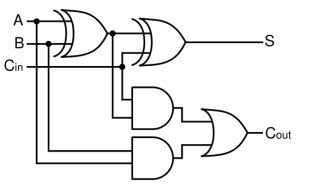
\includegraphics[scale=0.5]{HAFA}
 \caption{Full adder block diagram}
\end{figure}
\newpage
The Full Adders were connected like this:\\

\begin{figure}[H]
 \centering
 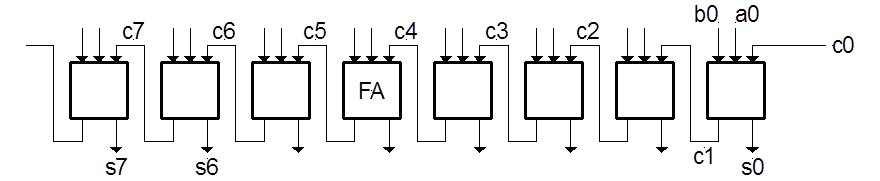
\includegraphics[scale=0.3]{RCA}
 \caption{RCA made from FA blocks}
\end{figure}

We designed it like this since this was the only logic way of using the FA:s as a RCA. 
When doing the RCA, we learned how to use portmaps and how signals work in VHDL.

\subsubsection{CMP}
We designed the CMP-unit using a ERMWAT, since we only needed to compare two signals, and thus, it wasn't really that complex to implement using only gates.\\
For every bit of all both input-signals, we compared those using a XOR-gate. All these results were then put together using OR-gates. This result would be NEQ. The EQ was then acquired using NOT NEQ.


\subsubsection{4 to 1 multiplexer}
The multiplexer were implemented with a simple \emph{case}, which just decided wether to use the output from the RCA, the NAND- or the NOTsignal.

\subsubsection{ALU}
Four operations was supported:\\
\begin{center}
\begin{tabular} {|l|l|} \hline
operation & Operation \\
\hline 00 & Add  \\
\hline 01 & Sub \\
\hline 10 & NAND \\
\hline 11 & NOT \\
\hline
\end{tabular}
\end{center}

The interesting part is the subtraction. In that case, we inverted in-signal B, and added insignal A and the inverted B with the carry set. This resulting in adding in-signal A with the twocomplement of in-signal B, which is the same thing as subtraction.
Since the operation for Add was 00, and for Sub was 01, it was easy to decide when to use a carry-in for the RCA; it was the same as the LSB of the operation-code.

The other two operations, NAND and NOT, were simply saved as signals.\\
The Multiplexer then chose outputsignal of the ALU depending on the operation.\\

After designing all the components, we simply had to wire everything together, using the diagram provided.\\

When designing the ALU, we learned how an ALU works, nailed down to the smallest grinds. We also learned more about VHDL, how to design components, and how to use designed components together to build a more complex design.
\subsection{Top-level Design}

During this lab the goal was to complete the top level design of the ChAcc processor.
To be able to do this we had to use the modules from the previous along with a few new.\\

New modules that needed to be created for this lab:

\begin{itemize}
	
    \item Storage components(register and memory)
    \item The bus
    
\end{itemize}

\subsubsection{Register}

The register was built from a D flip-flop with an load enable signal that decided if the register should get a new value or keep the old one.
For the register we used DESIGNSTYLE!!!!! as designstyle.
Because the ChAcc uses registers with different bit-widths we had to make the module generic. The register module was tested successfully with a do-file.

\subsubsection{Memory}

The ChAcc needed two memories. One for instructions and one for data.
Both of them were build using them same memorymodule.
The memories was built as an twodimensional-array that had an adresswidth and a datawidth. Both of them with a generic size so different memories could be built with the same module. It also had an generic initialization file.//
The memory had a data-in-signal which contained the data you wanted to write to the memory. It also had an adress signal that contained the adress you wanted to write to or read from.
The data memory had an write enable (WE) signal that had to be set to write to the memory.
The instruction memory still had the WE, but it is never set since it is only required to read from it, and not write to it.

\begin{figure}[H]
 \centering
 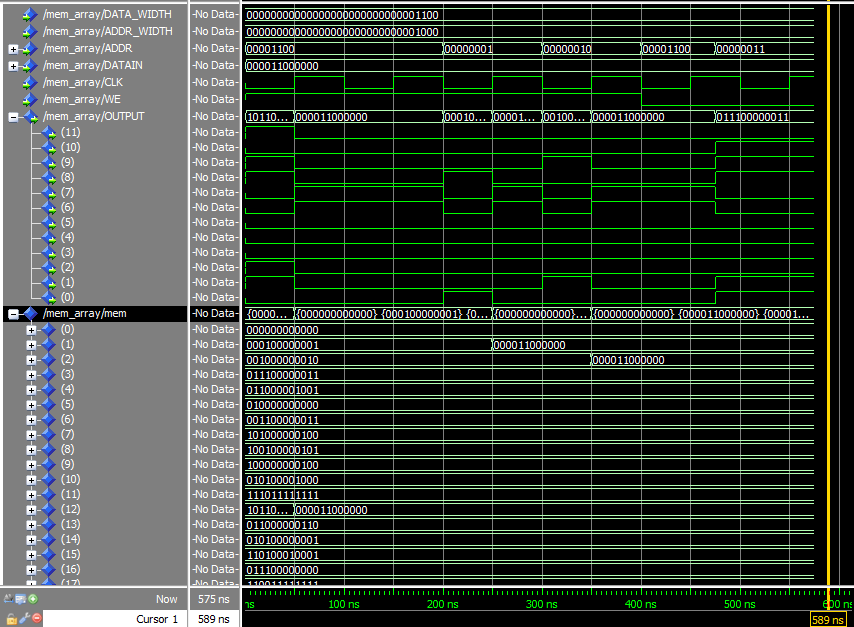
\includegraphics[scale=0.3]{lab3}
 \caption{Memory read/write test}
\end{figure}
			

\subsubsection{The bus}

The bus was implemented using the mux module from lab2.
Four muxes were used, each giving the bus a different output.\\

The following signal gave the following output on the bus:\\
\begin{center}
\begin{tabular} {|c|c|} \hline
Signal & Output on bus \\
\hline im2bus & addrFromInstruction\\
\hline dmRd & MemDataOutReged\\
\hline acc2bus & OutFromAcc\\
\hline ext2bus & extIn\\
\hline
\end{tabular}
\end{center}

If two or more signals were set at the same time an error output is set on the bus. This is to prevent several outputs to the bus at the same time.\\
\\
With these new modules we were able to write all the port maps to create the processor, except for the controller.

\subsection{Controller}
The controller consisted of 3 processes:
\begin{itemize}
 \item A process which clocked the controller, and updated the state.
 \item A process which calculated the next state depending on the current state.
 \item A process which set the right flags depending on the current opcode and state.
\end{itemize}

To design the second process, we had to draw a state diagram for the controller:\\



\begin{figure}[H]
\centering
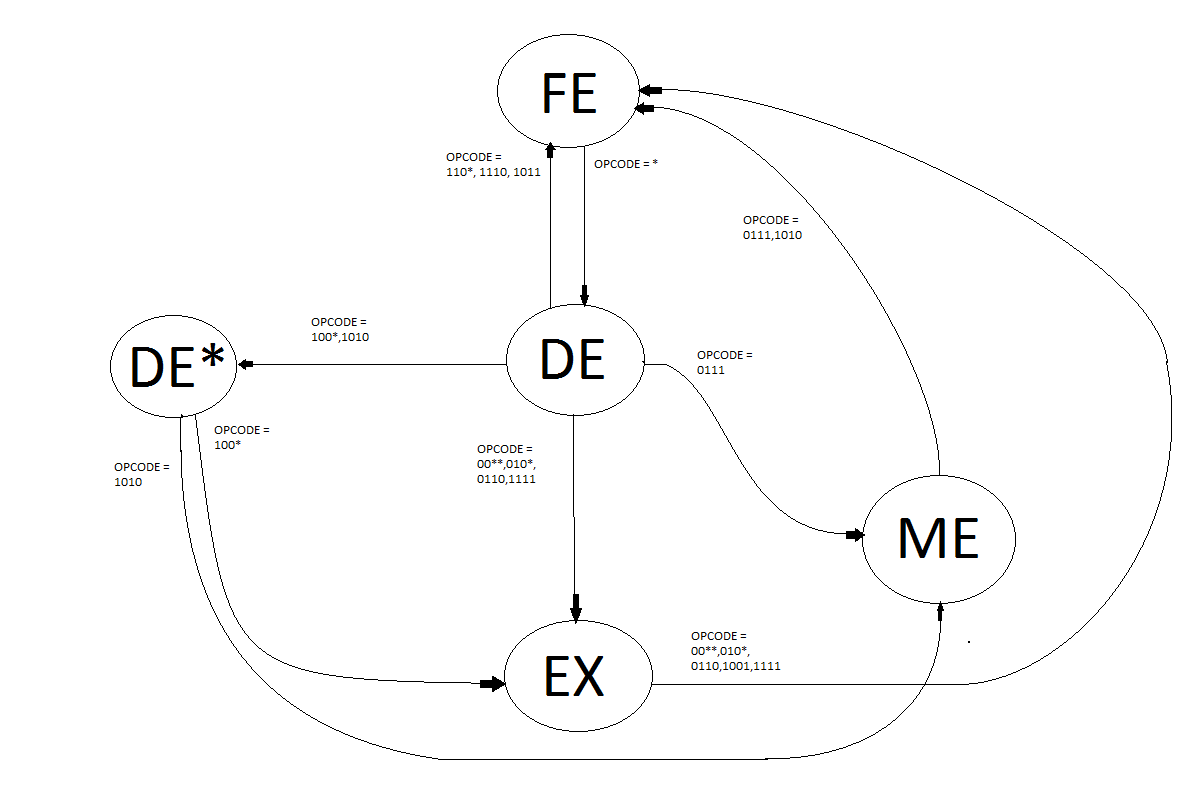
\includegraphics[scale=0.3]{FSM}
\caption{State diagram}
\end{figure}


When looking at this state diagram, it was much easier to see how we were supposed to design this process.

When designing the third process, a table of flags depending on what state and opcode was provided. But this table wasn't easy enough to follow, so we made our own table, which made much more sense:
\begin{center}
\begin{tabular}{|c|c|c|c|c|c|c|c|} \hline
 & FE & DE & DE* & EX & ME & ALLSTATES & aluMd\\
\hline 0000 && dataLd && \parbox{1.2cm}{pcLd, FlagLd, accLd, dmRd} &&& 00\\
\hline 0001 && dataLd && \parbox{1.2cm}{pcLd, FlagLd, accLd, dmRd} &&& 01\\
\hline 0010 && dataLd && \parbox{1.2cm}{pcLd, FlagLd, accLd, dmRd} &&& 10\\
\hline 0011 && dataLd && \parbox{1.2cm}{pcLd, FlagLd, accLd, dmRd} &&& 11\\
\hline 0100 && dataLd && \parbox{1.2cm}{pcLd, FlagLd, accLd, dmRd} &&& xx\\
\hline 0101 && dataLd && \parbox{1.2cm}{pcLd, FlagLd, dmRd} &&& xx\\
\hline 0110 && dataLd && \parbox{1.2cm}{pcLd, accSel, accLd, dmRd} &&& xx\\
\hline 0111 &&&&& pcLd, dmWr & acc2bus & xx\\
\hline 1000 && dataLd & addrMd, dataLd & \parbox{1.2cm}{pcLd, FlagLd, accLd, dmRd} &&& 00\\
\hline 1001 && dataLd & addrMd, dataLd & \parbox{1.2cm}{pcLd, accSel, accLd, dmRd} &&& xx\\
\hline 1010 && dataLd &&& \parbox{1.2cm}{pcLd, addrMd, dmWr} & acc2bus & xx\\
\hline 1011 && pcLd, dmWr &&&& ext2bus & xx\\
\hline 1100 && pcSel, pcLd &&&& im2bus & xx\\
\hline 1101 && pcSel, pcLd &&&& im2bus & xx\\
\hline 1110 && pcSel, pcLd &&&& im2bus & xx\\
\hline 1111 &&&& pcLd, dispLd &&& 00\\
 \hline
\end{tabular}
\end{center}

\subsubsection{Troubleshooting}
At first, the resulting datamemory didn't make sense at all, it seemed like nothing worked. After an hour of troubleshooting, we found that we forgot to initiate our data memory to read from the data\_mem file, so it defaulted to read from the instr\_mem, which made everything completely wrong.
After fixing that, a few timing issues was found in the processes; they weren't starting on the correct triggers. Fixing that made everything work correctly.

\subsection{Processor's Testbench}

During this lab we tested our final processor design.
For the test we used one intruction file, one data file and five trace files.
The trace files were read and stored in five different arrays.
The data and instruction file were read and stored in the data and instruction memories.\\
Five processes were created, each were triggered when the signal of interest changes.
When a process was triggered, it compared the signal value with an expected value from its associated trace file. What index in the trace file to compare with was decided by a counter; one for each process, that increases by one each time the process vas triggered.
If the vaules didn't match, the program would give an error message depending on what signal was wrong.\\
At first our design did not work. Our testbeanch gave us alot of errors on two signals and two signals updated very rarely. 
Then, step by step, when went back in our modules, trying to find what we made wrong.
We ran new tests with do-files on every module, trying to find our error.
After hours of testing and troubleshooting, we realized that we missed some logic in opcode 1111 in our controller. We had missed to check the state, so the flags were always set during that opcode, no matter what state the processor was in, which messed up everything.

\begin{figure}[H]
 \centering
 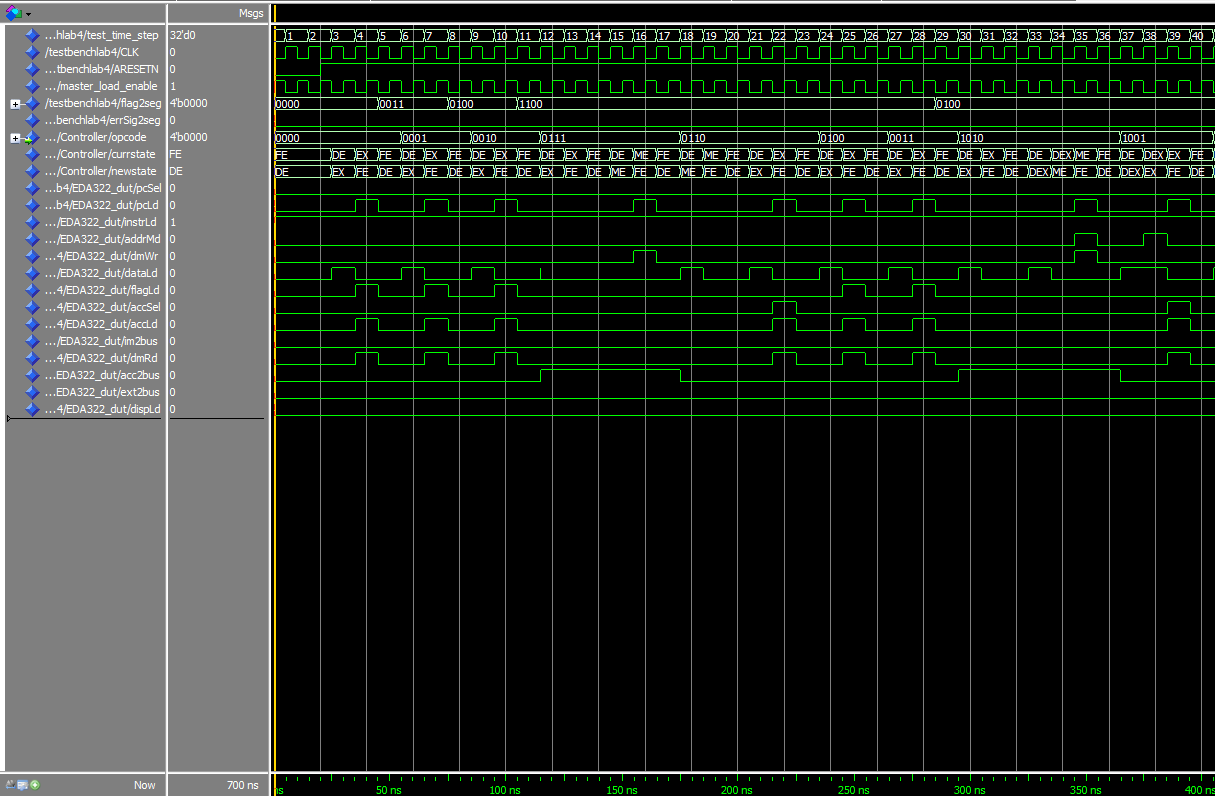
\includegraphics[scale=0.4]{lab4}
 \caption{Testbench result}
\end{figure}

\subsection{Analysis}

After the four labs we have managed to get a working and successfully tested processor.\\
It was interesting to get a better look of how a processor was designed and the different components that are mapped togheter to make it a fully working processor.
It also made us realize that small logical misstakes can create huge errors that takes a lot of time to fix, and in the begining it's hard to know where to start troubleshooting. Especially since a problem can first occur much later than expected if the testing of the component didn't cover all the cornercases.\\
The four labs have taught us about implementing different components using different designs styles and then port map them to create a working processor. We learned how to test our components and how to troubleshoot using waves to read values of signals.

\end{document}


